\chapter{Le projet de \textit{serious-game}}
Notre projet s'axe sur plusieurs parties, ayant pour but d'amener à la création d'un \textit{serious-game}, c'est à dire un jeu dont le premier objectif n'est pas le divertissement mais par exemple l'éducation ou l'exploration scientifique. Le projet se décompose en trois grandes étapes:
\begin{itemize}
\item{la réalisation d'un modèle à une espèce et la détermination des briques de bases de la simulation(caractéristiques des poissons et leurs interactions),}
\item{l'ajout de diverses espèces et d'interactions proies/prédateurs,}
\item{la recherche d'un état d'équilibre afin de pouvoir stabiliser l'écosystème créé,}
\item{enfin, l'ajout des pêcheurs et des ports.}
\end{itemize}

L'intérêt d'utiliser la forme d'un \textit{serious-game} est de pouvoir donner au joueur le pouvoir d'impacter la simulation, l'objectif étant une prise de conscience de l'impact de la pêche sur l'environnement, mais aussi du souci de la rentabilité. Le joueur doit réussir à mêler au mieux les deux pour réussir dans le jeu.

\section{Rapide présentation du \textit{serious-game}}

La simulation sur laquelle se base le \textit{serious-game} prend en compte plusieurs éléments. Il comprend les relations entre les proies et les prédateurs et la stabilité du système, les évènements ponctuels (tempêtes...) ainsi que l'impact de la pêche sur les populations marines selon les stratégies choisies.
\\
Le joueur doit gérer son parc de bateaux avec différent types de bateaux et les envoyer pêcher selon divers critères. Son but étant de pêcher le plus de poissons tout en minimisant les pertes (comme le fuel par exemple), le joueur doit comprendre l'impact qu'a les bateaux et les stratégies de pêche sur l'écosystème.
\\
Dans un second temps, chaque configuration possède un état stable dans lequel les poissons sont les plus nombreux et les mieux nourris. Dans le jeu, plus l'influence de la pêche sur cet environnement est élevée et moins le joueur gagnera de points.

\section{Représentation des ressources halieutiques par un \textit{serious-game}}

La représentation des ressources halieutiques\footnote{Les ressources halieutiques représentent l'art de la pêche et de la gestion des ressources aquatiques pêchées.} par un \textit{serious-game} nous permet d'avoir un "laboratoire virtuel", nous permettant de tester de nombreuses configurations. 
\\
Ces différentes configurations sont:
\begin{itemize}
\item{le choix des espèces représentées,}
\item{le choix des jeux de paramètres pour chaque espèce, chaque espèce étant représentée par sa consommation en nourriture, sa rapidité de reproduction, sa capacité à stocker de la nourriture et sa mortalité (en cas de manque de nourriture).}
\end{itemize}
Chaque espèce possède aussi une stratégie de migration, représentant sa capacité à trouver de la nourriture et à se disperser, ou alors rester grouper.
\\
Les différentes espèces de poissons sont représentées par sa masse (la \textbf{biomasse}). En effet celle-ci permet de représenter de manière simple et pertinente l'augmentation en taille des individus ainsi que l'apparition de nouveaux individus, ayant eux aussi leur masse propre.
\\
Ainsi, chaque interaction des poissons revient à créer un flux de biomasse d'un agent à un autre, ou bien tout simplement à représenter l'énergie dépensée par un évènement particulier.

\begin{figure}[h]
\begin{center}
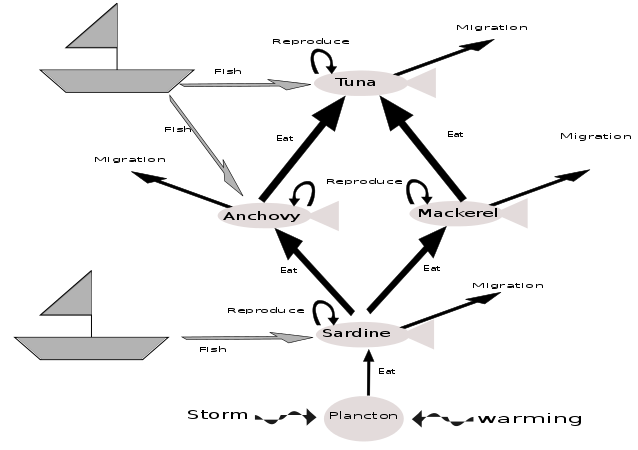
\includegraphics[scale=0.65]{img/flux.png}
\end{center}
\caption{Schéma représentatif des flux de biomasse}
\end{figure}

\section{Apport du système multi-agents pour la modélisation}

La plate-forme Netlogo spatialise les agents, ce qui permet de facilement gérer les déplacements d'un bateau d'un patch à un autre. Pour les poissons, chaque espèce a un seul et unique représentant (de l'intégralité des poissons de l'espèce présente) par case. Les différents agents agissent à chaque tour s'ils le peuvent avec les différents agents de la simulation, selon leurs besoins.
\\
On peut aussi observer l'impact spatial avec la répartition des différents agents selon leurs stratégies, diverses pressions (comme la pêche) et événements.
\\
Les différents agents ne peuvent interagir avec l'environnement et les autres agents que par des interactions dans notre modèle. Les agents représentant les poissons ont tous les mêmes interactions, ce qui permet de faciliter le développement en utilisant une interaction générique qui va être exécuté par tous les agents voulant l'implémentant. Cela nous a ainsi permis de développer les interactions selon un modèle simple (le plancton - \textit{Food} dans la simulation) et de généraliser vers le modèle complet avec différents agents proies/prédateurs.
